% Intended LaTeX compiler: pdflatex
\documentclass[10pt,a4paper,UTF8]{article}
\usepackage{zclorg}
\usepackage{tikztheorem}
\author{emacsun}
\date{}
\title{曲线拟合之最大斯然估计和最小二乘法}
\hypersetup{
 pdfauthor={emacsun},
 pdftitle={曲线拟合之最大斯然估计和最小二乘法},
 pdfkeywords={},
 pdfsubject={},
 pdfcreator={Emacs 25.2.1 (Org mode 9.0.9)},
 pdflang={English}}
\begin{document}

\maketitle
\tableofcontents
\titlepic{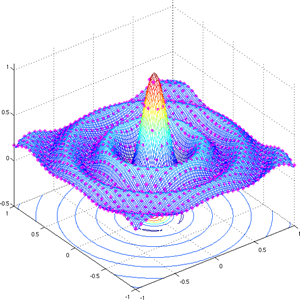
\includegraphics[scale=0.25]{../../img/sinc.PNG}}
\href{PRMLch1dot1-polynomial-curve.org}{之前},我们讨论过关于曲线拟合的一些概念,提到了均方误差函数和\href{PRMLch1dot1-polynomial-curve-probability-revist.org}{贝叶斯估计} , 并在一篇\href{PRMLch1dot1-polynomial-curve-matlab.org}{博文}中介绍了 matlab 实现。今天,我们讨论通过最小二乘法对最大斯然估计进行深入的挖掘。

\section{问题模型}
\label{sec:org4f0753a}


假设目标变量是\(t\),其可以通过如下模型生成:
\begin{equation}
\label{eq:1}
t = y(\mathbf{x},\mathbf{w}) + \epsilon
\end{equation}
其中,\(\epsilon\)是高斯白噪,均值为 0,方差是\(\beta\)。所以我们可以把\(t\)的概率密度函数表示为:
\begin{equation}
\label{eq:3}
p(t|\mathbf{x},\mathbf{w},\beta) = \mathcal{N}(t|y(\mathbf{x},\mathbf{w}),\beta^{-1})
\end{equation}
\section{问题分析:最大化斯然函数和最小化平方和误差函数的等效性}
\label{sec:orgd45cc90}


如果我们的损失函数是均方误差,那么对于一个新的输入\(\mathbf{x}\),最优的预测是基于目标变量的条件均值。针对式\textasciitilde{}(\ref{eq:3}),我们有:
\begin{equation}
\label{eq:4}
\mathbb{E}[t|\mathbf{x}] = \int tp(t|\mathbf{x})\mathrm{d}t = y(\mathbf{x},\mathbf{w})
\end{equation}
注意,高斯白噪的假设使得给定\(\mathbf{x}\)的\(t\)的条件均值是各向一致的。

现在考虑输入的数据集合\(\mathbf{X} = \{\mathbf{x}_{1},\ldots ,\mathbf{x}_{N}\}\),对应的目标变量是\(t_{1},\ldots ,t_{N}\)。我们假设数据集合是从式\textasciitilde{}(\ref{eq:3})所示分布中采样得到的。所以,关于\(\mathbf{X}\)的最大斯然估计为:
\begin{equation}
\label{eq:5}
p(\mathbf{t}|\mathbf{X},\mathbf{w},\beta) = \prod_{n=1}^{N}\mathcal{N}(t_{n}| \mathbf{w}^{T}\phi(\mathbf{x}_{n}),\beta^{-1})
\end{equation}
注意,这里我们假定 \[y(\mathbf{x},\mathbf{w}) = \mathbf{w}^{T}\phi_{x_{n}}\] 并且,我们不特别的约定基函数\(\phi(\mathbf{x})\)的形式。在监督学习问题中(分类或者回归),我们的目标不是为输入变量建模。\(\mathbf{x}\)会一直待在条件变量中,所以从现在开始我们去掉\(p(\mathbf{t}|\mathbf{x},\mathbf{w},\beta)\)中的\(\mathbf{x}\)。对式\textasciitilde{}(\ref{eq:5})求对数,把乘法变成加法,我们有:
\begin{equation}
\label{eq:6}
\ln p(\mathbf{t}| \mathbf{w},\beta) = \sum_{n=1}^{N}\ln \mathcal{N}(t_{n}| \mathbf{w}^{T} \phi(\mathbf{x}_{n}),\beta^{-1})
\end{equation}
对式\textasciitilde{}(\ref{eq:6})稍作变形,有:
\begin{equation}
\label{eq:7}
\ln p(\mathbf{t}| \mathbf{w},\beta) = \frac{N}{2}\ln (\beta) - \frac{N}{2}\ln(2\pi) - \beta E_{D}(\mathbf{w})
\end{equation}
其中,
\begin{equation}
\label{eq:8}
E_{D}(\mathbf{w}) = \frac{1}{2}\sum_{n=1}^{N}\{t_{n} - \mathbf{w}^{T}\phi(x_{n})\}^{2}
\end{equation}

我们发现,优化基于高斯白噪的斯然函数和最小化平方和误差函数是等效的。通过对\textasciitilde{}(\ref{eq:7})进行求导,有:
\begin{equation}
\label{eq:9}
\nabla \ln p(\mathbf{t} | \mathbf{w},\beta) = \sum_{n=1}^{N}\{t_{n} - \mathbf{w}^{T}\phi(\mathbf{x}_{n})\} \phi(\mathbf{x}_{n})^{T}
\end{equation}
令式\textasciitilde{}(\ref{eq:9})等于零,
\begin{equation}
\label{eq:10}
0 = \sum_{n=1}^{N}t_{n}\phi(\mathbf{x}_{n})^{T} - \mathbf{w}^{T}(\sum_{n=1}^{N}\phi(\mathbf{x}_{n})\phi(\mathbf{x}_{n})^{T})
\end{equation}
继而有:
\begin{equation}
\label{eq:11}
\mathbf{w}_{ML} = (\mathbf{\Phi}^{T}\mathbf{\Phi})^{-1} \mathbf{\Phi}^{T}\mathbf{t}
\end{equation}
这个解是最小二乘问题的解。这里\(\mathbf{\Phi}\)是\(N\times M\)的矩阵:
\begin{equation}
\label{eq:12}
\mathbf{\Phi} =
\begin{bmatrix}
\phi_{0}(\mathbf{x}_{1}) &  \phi_{1}(\mathbf{x}_{1}) & \ldots \phi_{M-1}(\mathbf{x}_{1})  \\
\phi_{0}(\mathbf{x}_{2}) &  \phi_{1}(\mathbf{x}_{2}) & \ldots \phi_{M-1}(\mathbf{x}_{2})  \\
\vdots & \vdots & \ddots & \vdots \\
\phi_{0}(\mathbf{x}_{N}) &  \phi_{1}(\mathbf{x}_{N}) & \ldots \phi_{M-1}(\mathbf{x}_{N})
\end{bmatrix}
\end{equation}
其中,\((\mathbf{\Phi}^{T}\mathbf{\Phi})^{-1}\mathbf{\Phi}^{T}\)是\(\mathbf{\Phi}\)的 Moore-Penrose 伪逆。这个伪逆是逆的推广。当\(\mathbf{\Phi}\)是方阵且可逆时,这个结果就直接等于\(\mathbf{\Phi}^{-1}\)

此刻,我们再分析\(w_{0}\)。重写\(E_{D}(\mathbf{w})\):
\begin{equation}
\label{eq:13}
E_{D}(\mathbf{w}) = \frac{1}{2}\sum_{n=1}^{N}\{t_{n} - w_{0} - \sum_{j=1}^{M-1}w_{j}\phi_{j}(\mathbf{x}_{n})\}^{2}
\end{equation}
对\(w_{0}\)求导,可得:
\begin{equation}
\label{eq:14}
w_{0} = \bar{t} -\sum_{j=1}^{M-1}w_{j}\bar{\phi_{j}}
\end{equation}
其中:
\begin{equation}
\label{eq:15}
\bar{t} = \frac{1}{N}\sum_{n=1}^{N}t_{n},\qquad \bar{\phi_{j}} = \frac{1}{N} \phi_{j}(\mathbf{x}_{n})
\end{equation}

所以,\(w_{0}\)补充了训练集合中目标值的均值与基函数之间的差值。

另外,我们可以对式\textasciitilde{}(\ref{eq:7})求\(\beta\)的导数,得\(\beta\):
\begin{equation}
\label{eq:16}
\frac{1}{\beta_{ML}} = \frac{1}{N}\sum_{n=1}^{N}\{t_{n}-\mathbf{w}_{ML}^{T}\phi(\mathbf{x}_{n})\}^{2}
\end{equation}
我们看到噪声精度的倒数是目标值在回归函数周围的方差。
\section{最小二乘的几何意义}
\label{sec:org3013812}


\begin{figure}[htbp]
\centering
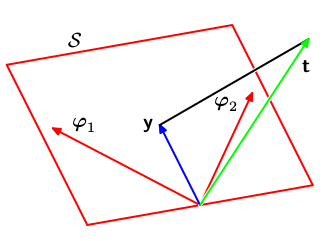
\includegraphics[width=0.6\textwidth]{../../img/computer_prml/20170806leastSquare.png}
\caption{\label{fig:orge1902c6}
最小二乘的几何意义}
\end{figure}

考虑\(N\)维空间,\(\mathbf{t}\)是其中一个矢量。每一个基函数\(\phi_{j}(\mathbf{x}_{n})\)取\(N\)个训练集合中的值也可以视作一个矢量,标记为\(\mathbf{\varphi}_{j}\),如图 \ref{fig:orge1902c6}所示。注意\(\mathbf{\varphi}_{j}\)对应\(\mathbf{\Phi}\)的第\(j\)列。如果基函数的个数\(M\)小于训练集合的点数\(N\),那么\(M\)个矢量\(\phi_{j}(\mathbf{x}_{n})\)张成一个\(M\)维的空间\(\mathcal{S}\)。我们定义\(\mathbf{y}\)是一个\(N\)维向量其第\(n\)个坐标为\(y(\mathbf{x}_{n},\mathbf{w})\)。因为\(\mathbf{y}\)是\(\mathbf{\varphi}_{j}\) 的线性组合。所以,\(\mathbf{y}\)可以在\(M\)维空间\(\mathcal{S}\)的任意位置。式\textasciitilde{}(\ref{eq:8})是\(\mathbf{y}\)和\(\mathbf{t}\)的欧几里得距离。所以\(\mathbf{w}\)的最小二乘解对应着\(\mathcal{S}\)中距离\(\mathbf{t}\)最近的\(\mathbf{y}\)。从图 \ref{fig:orge1902c6} 可以看出这个解对应着\(\mathbf{t}\)向\(\mathcal{S}\)的各个坐标系投影。

在实际应用中,直接求解\(\mathbf{\Phi}^{T}\mathbf{\Phi}\)的逆比较困难(因为,这个矩阵的维度比较大),所以一些数学技巧比如 SVD 分解经常会被用到。
\end{document}
